\chapter{Player Tracking}
\label{ch5}

In chapter~\ref{database}, a strategy was developed to determine which actions in the game cause which queries to the database. Further required tests were also discussed. 
In this chapter we look at methods available to gather player location data from the game. A specific method will then be chosen and every detail will be discussed and tested thoroughly. Other functions of player tracking software such as logging the location data, graphically displaying it and reading the logs will also be discussed in detail. 

\section{Different Methods}
This section discusses the different methods available to get the location data from players in WoW. The methods are then compared to each other to determine the best one to use.

\subsection{Server Side Tracking}
There are a few open source private WoW servers available online, such as ArcEmu, mentioned in chapter~\ref{ch3}. The server calculates the movement of all the NPCs and mobs in the game, and it receives all the locations from all the different clients too, which it sends back to all the clients for them to display. Since the private server is Open Source, the source code can be studied to determine where in the program the packets are handled. Extra code can then be added to the server to log all the location data for analysis purposes. 

%This method was disregarded without much consideration however, since the players need to be tracked on live servers, where server side access is not a possibility. Methods that are done on the client side are thus the only viable options.

\subsection{Intercepting Packets}
The client constantly sends updates of your current location to the server so that the server knows where you are in the game world. The locations of all the other players, NPCs and mobs that are in close proximity to your avatar (this is a radius of about 230 meters in-game) are also constantly sent to your client by the server. Before the client or server sends this information, it is encrypted. This is illustrated in figure~\ref{encryption}.

\begin{figure}[htbp]
\centering
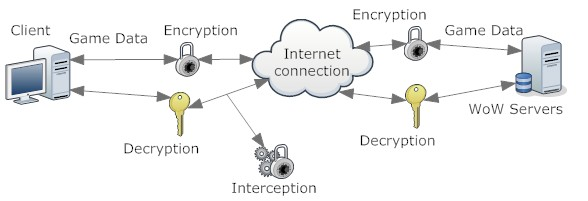
\includegraphics[scale = 0.6]{encrypt.jpg}	
\caption{WoW Server-Client Communication}
\label{encryption}
\end{figure}

The encryption and decryption is done in the client, so all intercepted packets will still be encrypted. WoW used XOR encryption on its header files since its release up until version 3.0.9. This encryption is not very secure and was easy to decrypt~\cite{xor}. The method of intercepting packets was done by~\citet{previous} to do their study on player movements in battlegrounds. 

WoW changed the form of encryption used with the release of patch 3.1.0 to RC4, which is a more secure form of encryption~\cite{rc4}. It is still possible to decrypt packets that are encrypted with RC4, but the key first needs to be found in memory. %Fortunately there are other methods available which also make use of memory reading that are much simpler, which is why this method was discarded.

\subsection{Reading Decrypted Packets}
When the client has decrypted the packets, they are moved to a set place in the clients memory where the client has to decide what the decrypted packets mean and what to do with them. By reverse engineering the WoW.exe file, this specific location in memory can be located and the decrypted packets can be read from the client's memory. This method is very viable, but a lot of the packets that are received will contain irrelevant information. The program will need to inspect every received packet and filter out the relevant ones for further analysis. %This method was discarded because there is a simpler and more efficient method available, discussed next.
Figure \ref{methods} shows visually where the decrypted packets are located that can be read.

\begin{figure}[htbp]
\centering
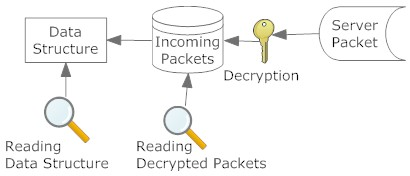
\includegraphics[scale = 0.65]{methods.jpg}	
\caption{Two methods of getting player location data}
\label{methods}
\end{figure}

\subsection{Reading WoW Data Structure}
The decrypted packets are all read by the WoW client to determine what they are for. When the client knows what a packet is for, it sends the packet on to where ever its right place in memory is. This process sorts all the received data into its right place in the WoW data structure. By reverse engineering the client, the data structures can be deciphered as well as the memory locations of the sorted data. All the data about players, NPCs and objects within visual range of your character in the game is sent to your client. That data is stored in memory, and can be read with the knowledge gained from reverse engineering the client. The data can then be displayed or stored after reading it. Figure~\ref{methods} shows where the data structure can be read from packets the server sends.

\subsection{Comparison}
The point of all these different methods of gaining the location of players is to be able to save and analyse the data to create movement models based on the movement of real people. The only place to gain meaningful movement data from WoW is by logging the movement of players on the live servers provided by Blizzard. 
The first method described requires access to the source code of the server to work. This method can thus be disregarded from the start, since access to the server is blocked. Only client-side tracking is considered viable.

The remaining three methods all require a program to read information from the client's memory. Intercepting the packets while they are still encrypted creates a lot of unnecessary effort if the memory is going to be read anyway. The second method of reading all received packets from memory gives exactly the same data as the first method of decrypting all received packets, but without the need to decrypt anything. Reading the received packets from memory is thus a better option than intercepting the encrypted packets. 

The method of reading the data structures of WoW from the client memory gives direct access to relevant data. Knowledge of the data structure used by WoW allows you to read the location data of players directly where it is stored. This method is better than reading all of the packets, where a lot of irrelevant data has to be sorted through. The method of reading the data structure is considered to be the best option available and is the method that will be used in this project.

%gaan soek wanneer encryption verander het. add references vir feite

%Discuss the different methods available, and briefly mention their complexities and difficulty. Motivate why you chose the method you chose.

\section{WoW Internal Data Structure}
Most programs use data structures to work with the variables needed to perform their different tasks. These include arrays, trees, structs, linked lists and so forth. With proper knowledge of how a program's data structures work, other programs can gain access to its data and functions by reading from and writing to the proper places in memory. When the source code of a program of interest is hidden, programmers use programs called disassemblers to gain information about the data structures of the program of interest. This is a complex and time consuming task, especially when there is a lack of previous knowledge of the program being disassembled. 

WoW is a very popular game however, and the gaming community has studied its data structures in fine detail. There is thus a lot of information available online on how to look for the right addresses to WoW's data structures, their respective sizes and how they link together. %The procedure to follow to find one address will be briefly discussed ~\cite{idapro}.
There are also many tutorials available online that show you how to reverse engineer WoW to gather this information~\cite{idapro}, but that is outside the scope of this project. Fortunately all the necessary information is usually posted on public forums such as www.ownedcore.com on the same day that a new patch is released.

\subsection{ASLR} %die subsection is dalk nie nodig nie?

Up until version 3.x of WoW, the base address of the process was always located at address 0x401000 in memory~\cite{wowbase}. This allowed programmers to use absolute addresses to all the data structures they wanted to access. The developers of WoW changed this from version 4.x onwards by adding support for address space layout randomisation (ASLR), to make WoW more secure. 

ASLR is security technology that makes a system more secure by making it harder for attackers to exploit existing vulnerabilities in the system. This is accomplished by randomising the memory layout of an executing program, which means that where an attacker could previously know exactly where a function would be in memory, the attacker would now have to guess the location in memory. This significantly decreases the chances of a single exploitation attempt being successful. It can also cause the program to crash, which limits the amount of exploitation attempts the attacker can practically make. ASLR is integrated into several operating systems, and is enabled by default in Windows Vista and Windows~7~\cite{aslr}. 
%soek references!

%gan maybe meer in detail in oor ASLR later?

%To decompile an executable file, the first thing you need is decompiler software. For this example, IDA Pro Disassembler will be used. The steps needed next are listed below:

%\begin{enumerate}
%	\item Open IDA Pro with administrator rights, and load the WoW.exe file into the program by clicking on File and Open.
%	\item A popup window should display after clicking open, where you should select the Portable Executable (PE) option.
%	\item After IDA has disassembled the binary it will show you a view of some subroutines and their addresses, which is not of much help. The best place to start looking is in the ``Strings Window''. To access this window, press ``Shift + F12''. This window will be used to search for something familiar.
%	\item Press ``Alt + T'' to search for a specific string, for this example search ``GetMinimapZoneText''. The program should now resemble Figure \ref{idascreen}.
	
%	\begin{figure}[htbp]
%\centering
%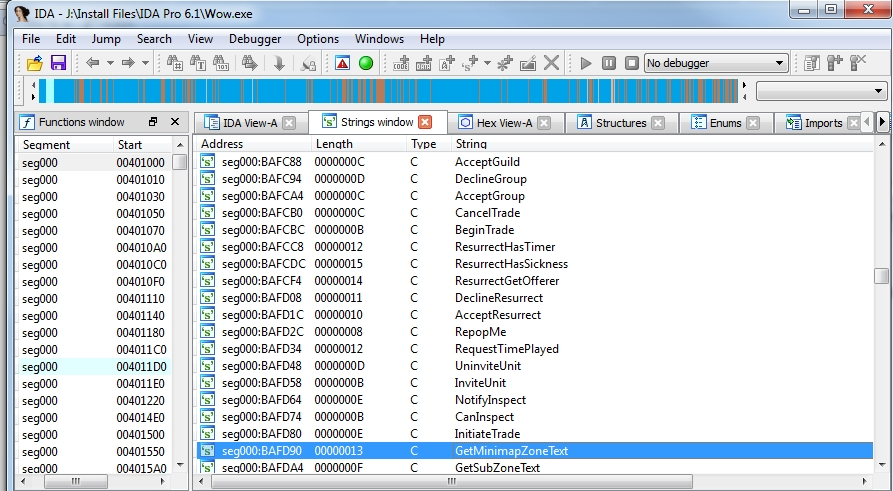
\includegraphics[scale = 0.6]{disassembled.jpg}	
%\caption{Typical Strings Window in IDA Pro}
%\label{idascreen}
%\end{figure}
	
%	\item Double clicking the ``GetMinimapZoneText'' line in the program will show you the ``IDA View-A'' of the code.
	
%\end{enumerate}

\subsection{Data Structures}

Extensive research has been done by the gaming community on exactly how the data structures of WoW works. The data structure of WoW is large and has information about everything that appears in the game. An overview of the complete data structure of WoW would contain a lot of data that is irrelevant to this project, therefore a simplified version that only includes relevant data will be provided here. All this information is the result of the hard work by people who reverse engineered WoW, and the validity of the data was confirmed by research done in the Memory Editing section of the OwnedCore forums~\cite{objman} and through thorough testing of the code.

The starting point and entry into the WoW data structure is the base address. This address can be found by searching for the base address of the process called wow.exe during runtime, which is the easiest way to circumvent ASLR. The WoW community have come up with a set of names for certain parts of the data structures to make sharing the offsets to those structures easier and more readable for everyone. The data structures are all tied together by offsets added together to create pointers to the actual data. This can become complex, with pointers pointing to pointers that finally point to the data that is needed.

Using the base address of the WoW process as starting point, access to some data can be gained by adding offsets to the base address and then reading that address. Here is a list of relevant information that can be gained directly by adding offsets to the base address of WoW and then reading that address:

\begin{enumerate}
	\item The name of your current player.%Base + playerName = Current Player Name. This address must be read as a string.
	\item The globally unique identifier(GUID) of your currently selected target in the game.%Base + LastTargetGUID = Globally unique identifier of your current target in the game. This must be read as an unsigned 64-bit integer and will return zero if no target is selected.
	\item An offset needed to access the object manager. This offset is called the client connection offset.%Base + clientConnection = ClientCon (address that needs to be added to another address to access the object manager). This must be read as an unsigned integer.
\end{enumerate}


There is a data structure in the WoW process that is referred to by the WoW community as the object manager. This data structure can be traversed similarly to a linked list once access to it has been gained, and it holds a list of all the WoW objects that are in close proximity to your character. It also stores many details about each object such as its name, type and location in X, Y and Z coordinates. Access to this data structure is thus exactly what is needed to extract the location data of all the players in close proximity to your character. 

\begin{figure}[htbp]  %maybe move figure to earlier in text.
\centering
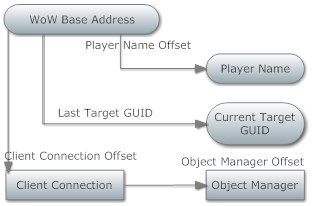
\includegraphics[scale = 0.65]{objmanonly.jpg}	
\caption{How to access the object manager}
\label{datastruct}
\end{figure}


As can be seen simplified in figure~\ref{datastruct}, access to the object manager can be gained by adding the client connection offset to the object manager offset and reading that address. This is then the base address of the object manager, which gives you access to two important things by adding two separate offsets to it. 

The first is your character's GUID, which is accessed by adding your local GUID offset to that of the base address of the object manager and reading it as an unsigned 64-bit integer.
The second is the base address of the first object in the object manager, which is accessed by adding the first object offset to the object manager base address and reading it as an unsigned integer.

Each object in the object manager has certain data fields that are consistent for all objects, whether it is gold, a human player or an NPC. These include its X, Y and Z coordinates as well as the rotation of the object, the GUID, and its type. It also has a pointer to what is called its object fields. The object fields contain some data about the object that is also contained within the normal object structure such as its type and GUID. This fact makes it easy to test if a program is reading the data correctly by comparing the repeated values. If the object is a player, the object fields also contain a lot of data about the player such as the health, mana and so forth.

The object type field tells you what kind of object you are working with. If the value returned is 3 it means the current object is an NPC, while a value of 4 means that it is a human player. The other types of objects are not relevant to this project and will not be discussed. 

The next object in the object manager can be accessed by adding the next object offset to the current object. This can be repeated until null is returned, which indicates the end of the list of objects.
A graphical representation of the object manager data structure is shown in figure~\ref{objalone}.

\begin{figure}[htbp]  %maybe move figure to earlier in text.
\centering
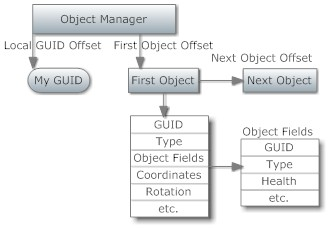
\includegraphics[scale = 0.65]{objmanalone.jpg}	
\caption{A representation of the object manager}
\label{objalone}
\end{figure}

%Discuss ASLR, Warden. Explain how objects are related to each other in WoW memory space. Also mention how they change with every update. Explain how to reverse engineer the client to get this structure when its updated briefly and where it is available online after its updated.
\lstset{language=c}
\lstset{basicstyle=\small}
\lstset{backgroundcolor=\color{listinggray},rulecolor=\color{blue}}
\lstset{linewidth=\textwidth}
\lstset{commentstyle=\textit, stringstyle=\upshape,showspaces=false}
\lstset{frame=trBL,frameround=tttt}


\section{Tracking Software Logic}
In this section, the logical flow of the tracking software implemented in this project is discussed in detail. The features needed by the program is first discussed, before giving an overview of the program  in the form of a flow diagram, with each of the more complex blocks being discussed in more detail further on in the section.

\subsection{Features Needed}
When designing software from scratch, it is helpful to first imagine a scenario of a user using the software to determine what features the software needs to provide. The software also needs to anticipate any actions that an unknowing user could do to prevent errors from occurring. The following short scenario reveals a few things the software should anticipate, as well as the features that are needed.

When a user wants to gather location data in WoW with this software, his first steps would be to start both the tracking software and WoW. The tracking software will only be able to track players once the user has entered the game world fully however, so a message should be displayed informing the user to click a reload button once the game world has been entered. The first potential problem the user could have is that the tracking software window is hidden behind the game window. This suggests that an option is needed to keep the tracking software window always on top.

Now that the program window is in view and has been loaded fully, the user needs some assurance that the program is working correctly. For this purpose a graphical representation of the player and surrounding NPCs and players need to be shown. Some information about the character of the user and the characters' current target being displayed will also assure the user that the program is working properly. A function is thus needed that draws players or messages on a bitmap that is then displayed to the user.

The user should now be convinced that the program is working and would want to start using it for tracking purposes. The user might only want to capture location data at certain times, so the option to turn tracking on and off is needed. The tracking data can be used in many ways, but the most obvious way would be to plot traces of the movement data captured. It would be very convenient for the user to not only have the option of tracking players, but to also show the traces as they happen in real time as a visual representation of the players being tracked. The user would then want to save the data to files when the tracking is done, before exiting the program and WoW.

From this scenario it is determined that the software needs the following features:

\begin{itemize}
	\item A reload button in case the user opens the program too soon, or something goes wrong.
	\item An option to keep the tracking window on top of other windows.
	\item An option to start and stop tracking players.
	\item An option to show the traces of players as they move.
	\item A button to save the tracking data when the user is done tracking.
\end{itemize}

Some features are only realised as the program progresses. Using the software showed that the graphical representation of players can become unusable when too many players are cluttered together. A zooming feature was added to add space between players in cluttered areas. An option to hide names from the graphical representation was also added to cause less clutter. Figure~\ref{wowdar1} shows the final GUI for the tracking software.

\begin{figure}[htbp]  %maybe move figure to earlier in text.
\centering
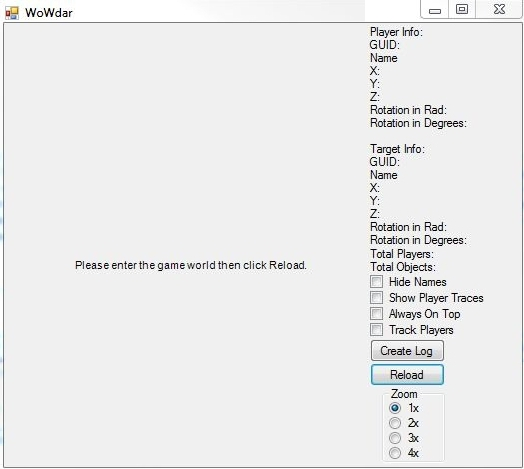
\includegraphics[scale = 0.65]{wowdar.jpg}	
\caption{The user interface of the tracking software program}
\label{wowdar1}
\end{figure}

\subsection{Initialisation}

The software needs to know when the user selects one of the features. To be able to do this a logical flow of events is needed in the software.

The first step for any software is to initialise the program. After initialisation the program needs to know if it loaded successfully or not, it also needs to let the user know this. The initialisation process of the program only involves loading the values of some needed global constants from the memory of the WoW client. The program then sets a flag true if the initialisation succeeded or false if it failed. The end of the code is then reached and the program stops temporarily.

The simplest way to describe the nature of the program is that it has to read values over and over again. This means that one block of code needs to be executed infinitely while the program is running, to keep the data up to date. To do this, a timer is needed. The timer is set to generate an interrupt every 10 milliseconds (ms) and to execute a block of code every time an interrupt is generated. 

Two flow diagrams are thus needed for this program, one for the initialisation and one for the code that gets executed every 10 ms. On overview of the initialisation code is shown in figure~\ref{init}.

\begin{figure}[htbp]  %maybe move figure to earlier in text.
\centering
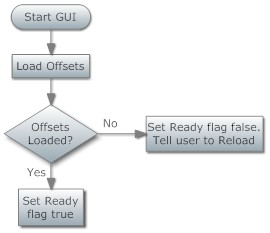
\includegraphics[scale = 0.65]{initover.jpg}	
\caption{An overview of the initialisation process}
\label{init}
\end{figure}

\subsection{Loading Offsets}

The Load Offsets block in figure~\ref{init} is a function that needs further explanation. The job of the Load Offsets function is to read a few values out of the WoW client software memory and to save it as global constants. These constants are needed by the code that executes every 10 ms to be able to access the object manager among other things.

The first problem this function has is that it needs access to the base address of WoW. The whole point of ASLR is to make sure that the base address is always different, so it needs to find another way to get the base. To get the base address of a process that uses ASLR, it is necessary for the process to be executed and loaded into memory first. Every process that is currently running is given a process identifier (PID) by the operating system to distinguish between different processes. The Load Offsets function searches through the list of running programs for one that is called WoW. Once it has the PID of WoW, C\# provides methods to get the base address of the process.

The Load Offsets function then adds a few different offsets to the base offset of WoW to get access to the following constants:
\begin{itemize}
	\item The base address of the object manager.
	\item The base address of the first object in the object manager.
	\item The GUID of the currently selected target.
	\item The GUID of the current character.
	\item The name of the current character.
\end{itemize}

The function then changes the labels on the GUI to show the name and GUID of the current character. The function returns true if all of this was done successfully. If any of the above steps failed however, the function informs the user that the Reload button must be clicked once the game world has been entered, and returns false. A flow diagram of the Load Offsets function is shown in figure~\ref{loadoff}.

\begin{figure}[htbp]  %maybe move figure to earlier in text.
\centering
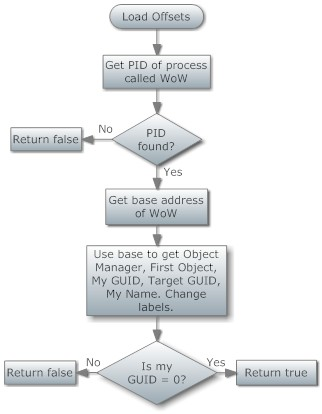
\includegraphics[scale = 0.65]{loadoff.jpg}	
\caption{A flow diagram of the Load Offsets function}
\label{loadoff}
\end{figure}

After the initialisation has taken place, the timer is started and after 10 ms the recurring code is executed for the first time. The program needs to be aware of any options chosen by the user, so a test is required to determine which options are selected. The user will see how the program reacts by the way that the user's character and other players and NPCs are sketched on the bitmap. It is thus important that the program reacts immediately when an option is changed.

\subsection{Recurring Code}

The first thing the recurring code needs to check is whether the initialisation was successful. If it was not, the user needs to be informed that the Reload button must be pressed with a message written on the bitmap. If the initialisation was successful, the program needs information that will determine how the players are drawn on the bitmap. This includes information such as the zoom level chosen and whether player traces must be shown or not. When the option to display traces is selected, the usual arrow used to display players is replaced by a thin line. All names are also hidden automatically in this view, and the bitmap is never cleared in order to keep previous traces of players. If the option is not selected however, the bitmap must be cleared to update the positions of all the players.

After checking which visual options are chosen, the program needs to get gather the necessary information to display all the characters in the game. It does this by using the global constant values which the initialisation process read from memory. 

Before the program goes on to read all the needed information from memory, a data structure needs to be defined in which all this data can be grouped together and saved. A class called WoW Object is created for this purpose, with fields to save the GUID, name, type, base address, object fields base address, health, coordinates and rotation in one data structure. Figure~\ref{wowobject} shows the WoW Object data structure.

\begin{figure}[htbp]  %maybe move figure to earlier in text.
\centering
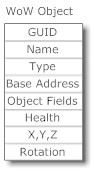
\includegraphics[scale = 0.65]{wowobject.jpg}	
\caption{The WoW Object data structure}
\label{wowobject}
\end{figure}


The program starts by saving the base address of the first object in a temporary variable to be used later. It also reads the GUID of the currently selected target again in case it changed since either initialisation or the previous 10 ms code execution. One of the global constants is the GUID of the local character. This GUID can be used to get the base of the local character object, which in turn grants access to the coordinates and rotation information. This information is then saved in a WoW Object for later use.

The next object of interest is our current target if one is selected. If no target is selected then the target GUID would be zero and the program would skip on. If there is a target currently selected however, then the GUID can once again be used to get the base address, which would grant access to the coordinates and rotation of the target. The target has more useful information which must also be read however, such as its type. Once the target has been classified as either human or NPC, the name of the target is read from memory, and all the information is saved in a WoW Object.

After the two special WoW Objects have been taken care of, the program needs to go through all of the other objects in the object manager and check the settings selected by the user each time to know what to do with the object. These objects are then drawn based on the selected settings one by one as the program loops through all the objects in the object manager.

After this process the program comes back to the two objects that are of special interest - the local character and the currently targeted character. The name and coordinates that was saved in WoW Objects for these two characters are then displayed on labels in the GUI, and the target and local player are sketched lastly on the bitmap, so that they would appear on top of the other objects if the other objects were close enough for them to overlap. Figure~\ref{10ms} shows an overview of this entire process.

\begin{figure}[htbp]  
\centering
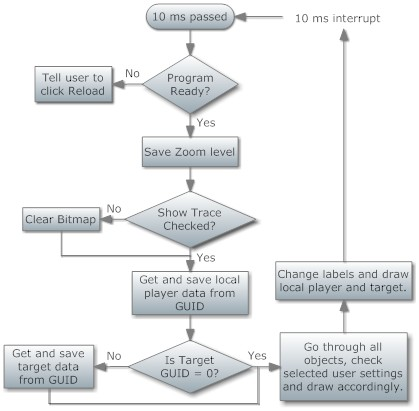
\includegraphics[scale = 0.65]{10ms.jpg}	
\caption{An overview of the code executed every 10 ms}
\label{10ms}
\end{figure}

Some of the blocks in figure~\ref{10ms} have more complex dynamics at work and need to be expanded into block diagrams of their own. When the program uses the globally constant local GUID to find the local player base, it is really calling a function to do this task. This function takes a GUID as an argument and returns the base of the object with the same GUID. It accomplishes this by using the globally constant value of the base address of the first object. 

It first compares the GUID received as argument to the GUID of the first object. If they match, the base address of the first object is returned. If they do not match, the algorithm moves on to the next object in the object manager and compares their GUIDs. This process is repeated until a match is found, or the end of the object manager is reached. If no match is found by the time the end is reached, zero is returned. Once the base address is returned, getting more information about an object is trivial. Figure~\ref{getbase} shows a flow diagram of this function.


\begin{figure}[htbp] 
\centering
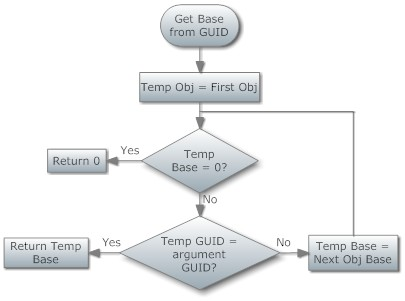
\includegraphics[scale = 0.65]{getbase.jpg}	
\caption{Flow diagram of get base by GUID function}
\label{getbase}
\end{figure}

\subsection{Cycling through the object manager}

The process of going through all the objects in the object manager, while checking which user settings are selected before drawing all the objects, was represented by a single block in figure~\ref{10ms}. This process is started by creating a WoW Object with the base of the first object. From the base, the other attributes of the object such as its GUID, coordinates, type and health is read by adding the appropriate offsets to the base address. The procedure for getting the name of an NPC is different from the one to get the name of a human player, so the type must first be analysed before the name is read from memory. Once all the attributes are saved in the WoW Object, the options selected by the user must be analysed so that the program knows what to do with the object. 

The first problem is that the current object might be the local player object. The local player is never tracked, and must be sketched last so that it appears on top of other objects, so it must be excluded from the start. Once the program ensured that the current object is not the local player, only two cases must be evaluated. The type of the object must be analysed, and any object that is not an NPC or human player must be discarded.

If the object is an NPC, then it must only be drawn if the show player traces option is not selected. When it is selected, only human players are of interest. The only other value of interest is the current health of the NPC to determine if the NPC is alive. If it is still alive, the NPC must be drawn in a plum colour, otherwise it must be drawn in grey to indicate that it is dead.

If the object is a human player the health must be checked first. The reason is that dead players are not tracked and will not create any traces, so they can be drawn immediately. If the player is alive the program must check whether the player must be tracked or not. If the ``Track Players'' option is checked then the player location data must be saved, otherwise the player must be drawn on the map. It is not necessary to check whether the player traces option is selected, as this is checked in the function that draws players on the bitmap. Figure~\ref{objects} shows a flow diagram of this procedure. To keep the flow diagram simple, the check for dead players was omitted, and it is implied that any object that is not a player or NPC is discarded.


\begin{figure}[htbp]  %maybe move figure to earlier in text.
\centering
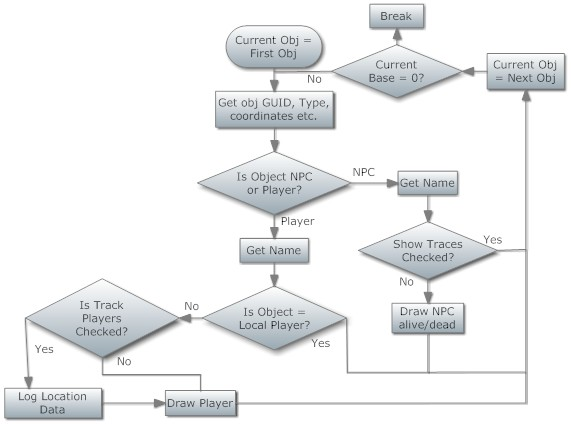
\includegraphics[scale = 0.65]{objects.jpg}	
\caption{Flow diagram of code that cycles through all objects}
\label{objects}
\end{figure}

%===================================================================================================================================================

\subsection{Logging information}
The end goal of logging the location data is to have the data saved for future use. This requires that the program either writes out the location data to a file every time it is read, or stores it in a data structure and writes it out when the user tells it to. Writing to a file takes more processing power than saving data in a data structure, which means that the first option would take more time to do than the second one, which could in turn cause the program to miss an update to the location data of a player.

For this reason a data structure is first needed to store all the relevant information in. For logging purposes the location of a unique player is important as well as the time when that player was at the specified position. The logs can then be used to completely reconstruct the movement of any player in exactly the same way that the player moved before, as well as in the same amount of time. To be able to save all this information, a structure called TimeAndPos is created with fields to save the location of a player and the time the player was at said location. 


The location of a player at a certain time is constantly changing, so all of this data needs to be stored in a list. This means that for every location and time pair of a player, a new structure must be created and stored. To order this information in a logical way, the structures are all placed in a list. The GUID of the player is not included in the TimeAndPos structure because the GUID of a player never changes and it would be a waste of resources to save the GUID over and over again.

To combine the list of movement data and the GUID of a player, a class called ObjArray is created. This class contains two fields: the GUID of one player, and a list called info, that contains all the TimeAndPos structures that form  a player's movement data in it.

The data structure described so far is suited to fully store the movement data of one player in WoW. There are many players that need to be tracked however, so the current data structure needs to be inserted into yet another list, which has one entry for every unique GUID.
A list called allObjects will be created for this purpose. Each entry in allObjects will thus contain a separate instance of the ObjArray class, with each one representing a unique player in the game world. The full data structure is represented schematically in figure~\ref{loggingstruct}.


\begin{figure}[htbp]  %maybe move figure to earlier in text.
\centering
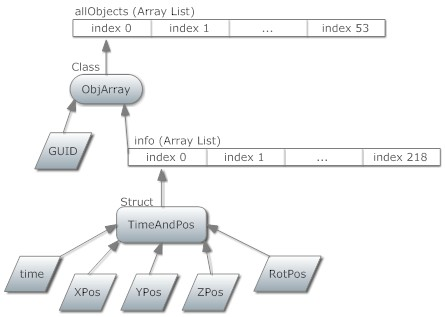
\includegraphics[scale = 0.65]{arrays.jpg}	
\caption{A schematic representation of the logging data structure}
\label{loggingstruct}
\end{figure}

The data structure shown in figure~\ref{loggingstruct} is needed to explain how the ``Log Location Data'' block in figure~\ref{objects} is executed.

At this point in the program, it has been determined that the ``Track Players'' checkbox has been checked and the location data needs to be logged. The program now has to save all the location data of the current player into the data structure shown in figure~\ref{loggingstruct}. The first step is to check if the list with all the objects in contains any data yet. 
If it does not, then that means that the current entry into it will be the first, and there is no need to search through it to see if the current player already has an entry in it. In this case the location data of the player and the current time must be added to the TimeAndPos structure, which must in turn be added into a new instance of the ObjArray class. The GUID of the player must then also be added to the ObjArray class, which is then inserted first into the list of all objects.

If there are already entries contained in the list, the program has to look through each entry in the list and compare the GUID contained in it to the GUID of the current object. If a match is found, the location data of the current object and the current time must be added to a new instance of the TimeAndPos structure, and added to the end of the info list. If the GUID is not found though, a new ObjArray instance must be created along with a new TimeAndPos structure. The data is then added into the TimeAndPos structure, which in turn is added to the ObjArray instance. The ObjArray is then lastly added into the allObjects list. Figure~\ref{logging} shows a flow diagram of this process.

\begin{figure}[htbp]  %maybe move figure to earlier in text.
\centering
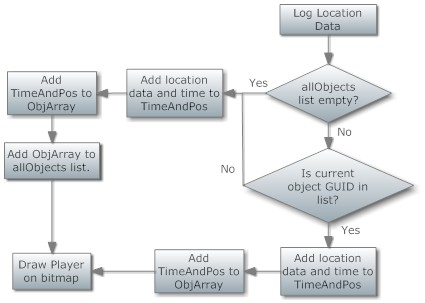
\includegraphics[scale = 0.65]{logging.jpg}	
\caption{Flow diagram of logging procedure}
\label{logging}
\end{figure}


At the moment all the data is saved in data structures, but as soon as the program is closed all this data will be lost immediately. The user needs to be able to choose when to save the data permanently. A button is provided in the GUI with the label ``Create Log''. When this button is clicked, all the data contained in the allObjects list needs to be saved to the computer in an ordered manner. A class called Log is created for this purpose. The class contains a method called WriteToFile, which takes the allObjects list as an argument and saves all the data contained in it to text files in the same directory as the executable file.

To distinguish between different players, the text file is named according to the GUID of the player. A possible name for a text file would be ``15543543556487.txt'' for example. This creates the potential problem that data from the same player might have been logged before, which could then be overwritten. To solve this problem the program will only append data to an existing file and create a new file if it does not exist  yet. All the data from previous logging sessions would  be unhindered with this method of saving. 

The data is written to the file with the date first, then the time of day accurate to 10 ms, then the X, Y and Z coordinates and finally the rotation. Each value is separated by a comma so that the data can easily be imported to programs such as MATLAB for further analysis.

%=====================================================================================================================================================

\subsection{Displaying player positions}


The virtual world in WoW is very large, and the Cartesian coordinates read from memory are usually large numbers. The only way to display characters from the game to the user in a intuitive and easy to understand way, is by displaying your own character in the center and then displaying all other characters relative to your own character. This is done by drawing all the characters on a bitmap, which is then displayed to the user.

The easiest way to sketch all the objects on one bitmap, is to create a function that takes the necessary data as arguments and returns a bitmap with the current player added to it. This function is then called after the data of each object in the object manager is read as can be seen in figure~\ref{objects}. When the end of the object manager is reached, the bitmap will be cleared unless showing player traces is enabled, and the process will repeat itself to show updated positions for all the players.

The following data is needed by the function:

\begin{itemize}
	\item The bitmap that must be drawn on. This bitmap must be a global variable.
	\item The colour to draw in.
	\item The Y-coordinate relative to your own Y-coordinate.
	\item The X-coordinate relative to your own X-coordinate.
	\item The rotation of the character in rad.
	\item The name of the player.
\end{itemize}

The coordinate system of a Bitmap object starts at zero in the top left corner, with the X-coordinate being more positive to the right, and the Y-coordinate being more positive to the bottom as shown in figure~\ref{bitmap}.

\begin{figure}[htbp]  
\centering
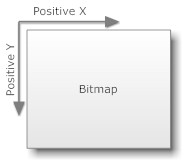
\includegraphics[scale = 0.65]{bitmap.jpg}	
\caption{The coordinate system of a Bitmap object}
\label{bitmap}
\end{figure}

This means that your character needs to be positioned at half the height and half the width of the bitmap in order to be displayed in the center. This offset needs to be added to the relative coordinates of any other characters as well in order to display correctly. The coordinate system used in WoW is inverted from the one used by bitmaps. In WoW the X-coordinate becomes more positive upwards, and the Y-coordinate becomes more positive to the right as illustrated in figure~\ref{wowcoord}.

\begin{figure}[htbp]  
\centering
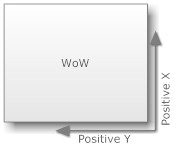
\includegraphics[scale = 0.65]{wowcoord.jpg}	
\caption{The coordinate system of WoW}
\label{wowcoord}
\end{figure}

If the X and Y-coordinates of the bitmap were switched around and then rotated 180 degrees, the two coordinate systems would be identical. For this reason, the X and Y-coordinates must be switched in the SketchPlayer function and the direction the character is looking in must also be rotated by 180 degrees. 

To rotate objects on a bitmap, a method called RotateTransform must be used. This method rotates an object by using the top left corner as its rotating axis, which creates a problem when the players need to be drawn in the middle of the bitmap. The only way to get around this problem is to first move the center point of the object, which is the relative coordinates in this case, to the top left corner. The object must then be rotated while it is in the corner by using the rotation information sent to the SketchPlayer function. After the object is properly orientated it must be moved back to its proper place. 

When these methods are used, it is technically the drawing coordinate system that is being moved around and rotated. This allows the function to move the coordinate system around before drawing the object on the bitmap, because once the object has been drawn it cant be changed without clearing the bitmap. The object is then only drawn after the drawing coordinate system is at the proper position. The program has to keep the user options in mind before drawing a player on the bitmap, by checking if the ``Show Traces'' option is selected. If it is, a line is drawn, otherwise an arrow is drawn.
The flow diagram of the SketchPlayer function is provided in figure~\ref{sketching}.

\begin{figure}[htbp]  
\centering
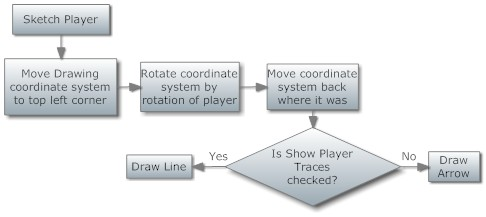
\includegraphics[scale = 0.65]{sketching.jpg}	
\caption{Flow diagram of the SketchPlayer function}
\label{sketching}
\end{figure}


%gaan nou in meer detail in oor die ander objects deel in, en dan meer, en meer. Maar eers get base by guid.

%\section{Memory Reading}
%
%In this section the procedure for accessing the memory of a process is discussed. This procedure is then expanded to include gathering the coordinates and other data from players in WoW. This knowledge was gained by studying similar open source projects that were done on previous versions of WoW, and applying modified versions of the same concepts to this project ~\cite{wradar, wowbot, wowradapp, wowradar}. 
%
%
%
%To be able to access the memory of a process, it is necessary for the process to be executed and loaded into memory first. Every process that is currently running is given a process identifier (PID) by the operating system to distinguish between different processes. The first step to accessing an open process is to get its PID. This can be done in C\# by using the Process.GetProcessesByName(String) method. 
%
%
%\lstset{language=c}
%\lstset{basicstyle=\small}
%\lstset{backgroundcolor=\color{listinggray},rulecolor=\color{blue}}
%\lstset{linewidth=\textwidth}
%\lstset{commentstyle=\textit, stringstyle=\upshape,showspaces=false}
%\lstset{frame=trBL,frameround=tttt}

%
%
%In the code, the Process.GetProcessesByName(string) method is called with the string ``wow'' as its argument. This returns an array of all processes with that name to the newly created wow process array. Usually only one instance of WoW is run on a computer at any one time, so the MainModule property of the first (and probably only) element in the array is assigned to the newly created ProcessModule object called ``wowModule''. Once we have the main module of the process, its simply a matter of assigning its BaseAddress property to a IntPtr object, and casting that object to an unsigned integer.
%WoWBase will now contain the base address of the WoW process.
%
%The .NET framework makes many of these types of operations easy to do, but there are open source libraries available that allows you to do these operations, and many others, with much less effort. The library used in this project is called ``BlackMagic'' and it makes process, thread and memory manipulation much easier and faster than it would normally be ~\cite{blackmagic}.
%The following code snippet shows how to get the  base address of the WoW process using the BlackMagic library.
%
%\begin{lstlisting}
%
%using System;
%using Magic;
%
%BlackMagic wow = new BlackMagic(); //create blackmagic object
%wow.OpenProcessAndThread(SProcess.GetProcessFromProcessName("Wow"))
%IntPtr baseWoW = wow.MainModule.BaseAddress;//Gets Base Address
%uint WoWBase = (uint)baseWoW;
%
%\end{lstlisting}
%
%This method is not all that much more efficient than the one using C\# libraries, but when it comes to memory reading, BlackMagic simplifies the process drastically. 
%
%When the needed information for each object is read from memory, the information needs to be stored in a structured way to make access to it easier. For this reason the WoWObject class is created with all the needed variables included. A code snippet of the WoWObject class is provided below.
%
%\begin{lstlisting}
%
%class WoWObject
%{
%   public ulong GUID = 0;
%   public String Name = "";
%   public short Type = 0;
%   public uint BaseAddress = 0;
%   public uint ObjectFields = 0;
%   public uint health = 0;
%   public float X = 0;
%   public float Y = 0;
%   public float Z = 0;
%   public float Rot = 0;
%}
%\end{lstlisting}
%
%Now that the base address of the process is stored and we have a class to store the needed values in, a few global constant values need to be read from memory and made available to the rest of the program. These include the base address of the object manager, the first object in the object manager, the GUID and name of your character, and the GUID of your characters' current target. The necessary offsets are all obtained from users who reverse engineered the WoW.exe file and posted their findings online, with the first and largest contributer mentioned as the source ~\cite{offsets}. The code needed to read the global constants from memory is listed below, with the relevant offsets included.
%
%\begin{lstlisting}
%
%uint ClientCon = 0;
%uint ObjectMan = 0;
%uint FirstObj = 0;
%
%WoWObject Me = new WoWObject();
%WoWObject Target = new WoWObject();
%
%//offsets for WoW 4.2.2.14545
%public enum ObjectManagerOff : uint
%{
%    clientConnection = 0x980558,
%    objectManager = 0x463C,
%    firstObject = 0xB4,
%    nextObject = 0x3C,
%    localGuid = 0xB8
%}
%    
%private Boolean LoadOffsets()
%{
%   ClientCon = wow.ReadUInt((uint)baseWoW 
%      + (uint)ObjectManagerOff.clientConnection);
%   ObjectMan = wow.ReadUInt(ClientCon 
%      + (uint)ObjectManagerOff.objectManager);
%   FirstObj = wow.ReadUInt(ObjectMan 
%      + (uint)ObjectManagerOff.firstObject);
%   Target.GUID = wow.ReadUInt64((uint)baseWoW 
%      + (uint)PlayerOff.LastTargetGUID);
%   Me.GUID = wow.ReadUInt64(ObjectMan 
%      + (uint)ObjectManagerOff.localGuid);
%   Me.Name = wow.ReadASCIIString((uint)baseWoW + 0x980598, 20);
%   
%   if (Me.GUID == 0)
%       return false;
%   else
%       return true;
%}
%    
%\end{lstlisting}
%
%It is clear from the code how easy and intuitive it is to read memory with the BlackMagic library.
%The constant values are used to gain access to all the objects in the object manager by cycling through them like a linked list. Even though the GUID of your character and your current target is already stored, the actual WoWObject of your character and current target which contains the location information is still in the object manager. A function is thus needed that takes a GUID as its argument and returns the base address of that object in the object manager. The function thus receives an unsigned 64-bit integer as argument, searches through all the objects in the object manager for an object with that GUID and then returns the base address of that object. The code that accomplishes this is shown below.
%
%\begin{lstlisting}
%
%public uint GetObjectBaseByGuid(ulong Guid)
%{  //start from first object
%   TempObj.BaseAddress = FirstObj;     
%
%	 //loop through all objects till right one is found
%   while (TempObj.BaseAddress != 0)    
%   {
%     try
%     {
%        TempObj.GUID = wow.ReadUInt64(TempObj.BaseAddress 
%           + (uint)ObjectOffsets.Guid, false);
%       if(TempObj.GUID == Guid)
%       {
%          return TempObj.BaseAddress;
%       }
%       TempObj.BaseAddress = wow.ReadUInt(TempObj.BaseAddress
%         + (uint)ObjectManagerOff.nextObject);    
%       //move on to next object
%     }
%     //must handle exception that can be thrown by blackmagic
%     catch (Exception)
%     {
%        return 0; //should never happen
%     }   
%   }
%  return 0;   //return 0 if nothing is found.
%}
%\end{lstlisting}
%
%A temporary object is created that takes on the value of the base address of the first object in the object manager. The offset needed to read the GUID of any object is then added to the base, and the GUID is read and compared to the GUID that was sent to the function. If the two GUID values are the same, the function returns the base address of the object. Alternatively the base address of the temporary object is changed to the base address of the next object in the object manager, and the procedure is repeated until the right object is found. If nothing is found, then zero is returned.
%
%This code is a good example of how to cycle through all the objects in the object manager, which needs to be done to get all the location information of all the players contained in it. Before the location information of other players are read however, the location of your own character is needed so that it is known where the other players are in relation to your own character. Getting this information is made easy by using the function listed above to get the base address of your character object, since the GUID is already stored. The code snippet that gets the rest of the relevant data from your character object is posted and explained below:
%
%\begin{lstlisting}
%  Me.BaseAddress = GetObjectBaseByGuid(Me.GUID);
%  Me.X = wow.ReadFloat(Me.BaseAddress + (uint)ObjectOffsets.Pos_X);
%  Me.Y = wow.ReadFloat(Me.BaseAddress + (uint)ObjectOffsets.Pos_Y);
%  Me.Z = wow.ReadFloat(Me.BaseAddress + (uint)ObjectOffsets.Pos_Z);
%  Me.Rot = wow.ReadFloat(Me.BaseAddress + (uint)ObjectOffsets.Rot);
%\end{lstlisting}
%
%The location information is stored as floats in WoW memory, and the Cartesian coordinate system is used for the X, Y and Z values, while the rotation float is stored in radians (rad). The location information of the current target is read in a similar fashion from memory and the code will thus not be reposted here. For any other object the reading process is slightly different however, since the type of the object must first be determined. The only objects that are relevant for displaying purposes are those of type three and four - NPCs and human players. Of those two types, only the human players will be tracked, but it is still useful to display positions of the NPCs for testing purposes. The code that reads this extra information from the WoWObjects follows:
%
%\begin{lstlisting}
%CurrentObj.GUID = wow.ReadUInt64(CurrentObj.BaseAddress 
%  + (uint)ObjectOffsets.Guid);
%CurrentObj.ObjectFields = wow.ReadUInt(CurrentObj.BaseAddress 
%  + (uint)ObjectOffsets.ObjectFields);
%CurrentObj.Type = wow.ReadShort(CurrentObj.BaseAddress + 0x14);
%CurrentObj.X = wow.ReadFloat(CurrentObj.BaseAddress 
%  + (uint)ObjectOffsets.Pos_X);
%CurrentObj.Y = wow.ReadFloat(CurrentObj.BaseAddress 
%  + (uint)ObjectOffsets.Pos_Y);
%CurrentObj.Z = wow.ReadFloat(CurrentObj.BaseAddress 
%  + (uint)ObjectOffsets.Pos_Z);
%CurrentObj.Rot = wow.ReadFloat(CurrentObj.BaseAddress 
%  + (uint)ObjectOffsets.Rot);
%CurrentObj.health = wow.ReadUInt(CurrentObj.ObjectFields 
%  + (uint)UnitFields.UNIT_FIELD_HEALTH);
%
%if (CurrentObj.Type == 3)    //NPC 
%{
%  CurrentObj.Name = MobNameFromGuid(CurrentObj.GUID);
%}
%if (CurrentObj.Type == 4)    //human player
%{
%  CurrentObj.Name = PlayerNameFromGuid(CurrentObj.GUID);
%}
%
%CurrentObj.BaseAddress = wow.ReadUInt(CurrentObj.BaseAddress 
%  + (uint)ObjectManagerOff.nextObject);
%
%\end{lstlisting}
%
%This code reads the object type, the object fields offset and then the health field contained in the object fields. The health field is read for displaying purposes, and to stop tracking players once they die. The method for getting the name of a player and a NPC is different, which is why different functions are needed to read that data. Those methods will be discussed later on in the text however. The relationship between all these fields are depicted clearly in Figure \ref{datastruct}.

%maybe add support for more than one wow process later
%Explain how to read from the game memory and to extract all the information needed. Also talk about the library used to do this, how it works and give credits to creator (shynd).

%\section{Tracking Software}
%In the previous section the code needed to access the location information for every object in the object manager was shown. Now that the program has a way of accessing all the location information, it needs ways to be able to log, display and save that information for future analysis. The program written for this project gives the user the option to track players, to hide object names and to show player traces. The programming behind these options will now be discussed in further detail. The different options available to users is shown in Figure \ref{wowdar}.
%
%\begin{figure}[htbp]  %maybe move figure to earlier in text.
%\centering
%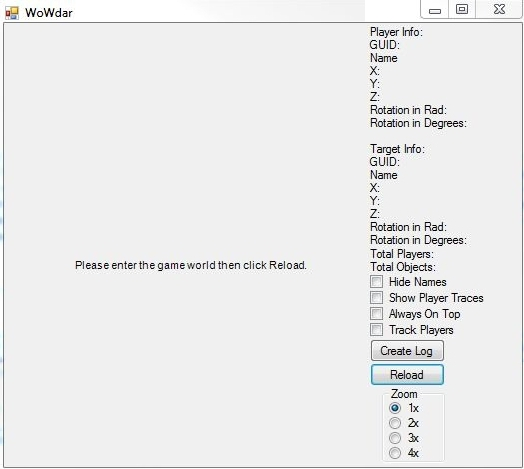
\includegraphics[scale = 0.6]{wowdar.jpg}	
%\caption{The user interface of the WoWdar tracking program}
%\label{wowdar}
%\end{figure}
%
%%Explain how the tracking software works briefly
%
%\subsection{Logging information}
%To be able to properly log the location information of players, a data structure is first needed to store all the relevant information in. For logging purposes the location of a unique player is important as well as the time when that player was at the specified position. The logs can then be used to completely reconstruct the movement of any player in exactly the same way that the player moved before, as well as in the same amount of time. To be able to save all this information a struct with the relevant fields mentioned above is created as follows:
%
%\begin{lstlisting}
%public struct TimeAndPos
%{
%  public DateTime time;
%  public float XPos;
%  public float YPos;
%  public float ZPos;
%  public float RotPos;
%}
%\end{lstlisting}
%
%The DateTime class allows the program to get and save the current time of the PC to the accuracy of a few milliseconds (ms). The time and location of a player will be changing constantly though, so all of this data needs to be stored in a list. The GUID of the player is also not included in this struct. The reason for that is that this struct will be in a list that will be growing constantly with updated information, while the GUID of a player will remain constant. Saving the GUID over and over again would be a waste of resources. A class with the name ObjArray is created to solve this problem. This class contains two fields in it: an unsigned 64-bit integer to store the GUID in, and an ArrayList object called info. The program reads the memory of WoW every 10 ms to update the location information of the objects in the object manager. Every time new information is read for a player, the program will store that information in a new instance of the TimeAndPos struct. This struct will then be added to the ArrayList called info, so that no information is lost. The ObjArray class is shown below:
%
%\begin{lstlisting}
%class ObjArray
%{
%  public ulong GUID = 0;
%  public ArrayList info = new ArrayList();
%}
%\end{lstlisting}
%
%There is still one problem that the data structure so far does not solve. The current setup only allows one GUID to be saved in the class. The info ArrayList contained in the class only has data that is relevant to the one GUID, so storing the other GUIDs in the ObjArray class is not an option. The solution is to create yet another ArrayList and to create a separate instance of the ObjArray class for each unique player. The ArrayList called allObjects will be created for this purpose. Each entry in allObjects will thus contain a separate instance of the ObjArray class, with each one representing a unique player in the game world. The full data structure is represented schematically in Figure \ref{loggingstruct}.
%
%
%\begin{figure}[htbp]  %maybe move figure to earlier in text.
%\centering
%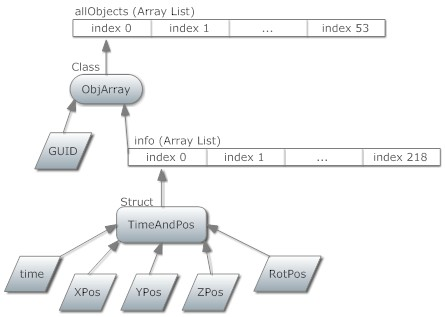
\includegraphics[scale = 0.6]{arrays.jpg}	
%\caption{A schematic representation of the logging data structure}
%\label{loggingstruct}
%\end{figure}
%
%The user is the one that controls whether the data must be logged or not. This is realised by only logging the data if the user selected the ``Track Players'' checkbox. When the checkbox is checked, the program will first test to see if the allObjects ArrayList contains any data. If it does not, then that means that the current entry into it will be the first, and there is thus no need to search through it for the current objects' GUID.
%
%If there are already entries contained in the ArrayList, the program has to look through each entry in the list and compare the GUID contained in it to the GUID of the object it is trying to add to the list. If they are the same, then the location information of the current object must simply be saved in a new instance of the TimeAndPos struct, and added to the end of the info ArrayList. If the GUID is not found though, then a new ObjArray instance must be created along with a new TimeAndPos. The TimeAndPos object is then added to the ObjArray instance, which is then added into the allObjects list. The relevant code section is posted below. This is after the program has confirmed that the current object is a human player that is not currently dead, and that the tracking checkbox has been checked.
%
%\begin{lstlisting}
%if (allObjects.Count <= 0)      
%{ //first entry into array
%  TimeAndPos temp = new TimeAndPos();
%  temp.XPos = CurrentObj.X;
%  temp.YPos = CurrentObj.Y;
%  temp.ZPos = CurrentObj.Z;
%  temp.RotPos = CurrentObj.Rot;
%  temp.time = DateTime.Now;       
%  ObjArray trackPlayer = new ObjArray();
%  trackPlayer.GUID = CurrentObj.GUID;
%  trackPlayer.info.Add(temp);
%  allObjects.Add(trackPlayer);
%}
%else                    
%{ //search through array for current player GUID
%  foreach(ObjArray tracking in allObjects)
%  {
%    if (tracking.GUID == CurrentObj.GUID) 
%    { //means current player GUID already in array
%      Found = true;
%      TimeAndPos temp = new TimeAndPos();
%      temp.XPos = CurrentObj.X;
%      temp.YPos = CurrentObj.Y;
%      temp.ZPos = CurrentObj.Z;
%      temp.RotPos = CurrentObj.Rot;
%      temp.time = DateTime.Now;
%      tracking.info.Add(temp);
%    }
%  }
%  if (!Found) //item not found in list, add it to list
%  {
%    TimeAndPos temp = new TimeAndPos();
%    temp.XPos = CurrentObj.X;
%    temp.YPos = CurrentObj.Y;
%    temp.ZPos = CurrentObj.Z;
%    temp.RotPos = CurrentObj.Rot;
%    temp.time = DateTime.Now;      
%    ObjArray trackPlayer = new ObjArray();
%    trackPlayer.GUID = CurrentObj.GUID;
%    trackPlayer.info.Add(temp);
%    allObjects.Add(trackPlayer);
%  }
%  else
%  {
%     Found = false;  //reset value for next object
%  }
%}
%\end{lstlisting}
%
%At the moment all the data is saved in data structures, but as soon as the program is closed all this data will be lost immediately. The user needs to be able to choose when to save the data permanently. A button is provided in the user interface (UI) with the label ``Create Log''. When this button is clicked, all the data contained in the allObjects ArrayList needs to be saved in text files on the computer in an ordered manner. A class called Log is created for this purpose. This class contains a method called WriteToFile in it. This method takes an ArrayList as an argument and saves all the data contained in it to text files in the same directory as the executable file.
%
%To distinguish between the different unique players, the text file is named according to the GUID of the object whose location information will be saved in it. An example name for a text file would thus be ``15543543556487.txt''. This creates the potential problem that data from the same player might have been logged before, and that data might then be overwritten. To solve this problem, the AppendText method of the File class in C\# is used. This method creates a file if it does not exist yet, and simply appends text to the end of the file if it does exist. All the data from previous logging sessions would thus be unhindered with this method of saving.
%
%The reason that the data is not saved to a text file every time new data arrives is that the writing operation takes much more central processing unit (CPU) processing time than adding the data to an ArrayList does. The code that saves the data to text files is shown below:
%
%\begin{lstlisting}
%public void WriteToFile(ArrayList datalist)
%{
%  foreach(ObjArray obj in datalist)
%  {
%    using (StreamWriter w = File.AppendText(obj.GUID + ".txt"))
%    {
%      foreach(TimeAndPos data in obj.info)
%      {
%        w.WriteLine(data.time.ToString("yyyy/MM/dd,HH:mm:ss.ffff") 
%        + "," + data.XPos + "," + data.YPos + ","+ data.ZPos + "," 
%        + data.RotPos);     //write data to log file
%      }
%      w.Flush();  //write and clear all buffered text
%      w.Close();  //close file
%    }
%  }
%}
%\end{lstlisting}


%moet dalk die kode uithaal later as daar min plek oor is (of verkort)
%Explain how the information is logged and saved for future use.
%Mention program that can read logs and refer to proper chapter.

%\subsection{Displaying player positions}
%The virtual world in WoW is very big, and the Cartesian coordinates read from memory are thus often big numbers. The only way to display characters from the game to the user in a intuitive and easy to understand way, is by displaying your own character in the center and then displaying all other characters relative to your own character. This is done in this project by making use of the Graphics class provided by C\#, and using it to draw on a Bitmap object which is then displayed to the user by using a picture box to display the bitmap.
%
%The easiest way to sketch all the objects on one bitmap is to create a function takes the necessary data as arguments and returns a bitmap with the current player added to it. This function can then be called after the data of each object in the object manager is read. When the end of the object manager is reached, the bitmap will be cleared and the process will repeat itself to show updated positions for all the players.
%
%The following data will be needed by the function as arguments:
%
%\begin{itemize}
%	\item The bitmap that must be drawn on.
%	\item The colour to draw in.
%	\item The Y-coordinate relative to your own Y-coordinate.
%	\item The X-coordinate relative to your own X-coordinate.
%	\item The rotation of the character in rad.
%	\item The name of the player.
%\end{itemize}
%
%The coordinate system of a Bitmap object starts at zero in the top left corner, with the X-coordinate being more positive to the right, and the Y-coordinate being more positive to the bottom as shown in Figure \ref{bitmap}.
%
%\begin{figure}[htbp]  %maybe move figure to earlier in text.
%\centering
%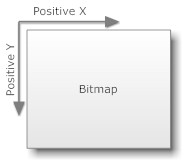
\includegraphics[scale = 0.6]{bitmap.jpg}	
%\caption{The coordinate system of a Bitmap object}
%\label{bitmap}
%\end{figure}
%
%This means that your character needs to be positioned at half the height and half the width of the bitmap in order to be displayed in the center. This offset needs to be added to any other characters relative coordinates as well to display correctly. The coordinate system used in WoW is a inverted from the one used by bitmaps however. In WoW the X-coordinate becomes more positive upwards, and the Y-coordinate becomes more positive to the right as illustrated in Figure \ref{wowcoord}.
%
%\begin{figure}[htbp]  %maybe move figure to earlier in text.
%\centering
%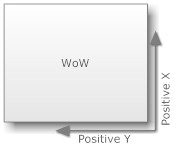
\includegraphics[scale = 0.6]{wowcoord.jpg}	
%\caption{The coordinate system of WoW}
%\label{wowcoord}
%\end{figure}
%
%If the X and Y-coordinates of the bitmap were switched around and then rotated 180 degrees, the two coordinate systems would be identical. For this reason, the X and Y-coordinates must be switched in the SketchPlayer function. The direction the character is looking in must also be rotated by 180 degrees. This is done using the RotateTransform method of the Graphics class. This method rotates the drawing coordinates from the left top corner of the bitmap. 
%
%This method also uses degrees as an argument, so the radians first needs to be converted to degrees. After this conversion is made, the coordinates where we want to draw must be moved so that it is in the top left corner first. The coordinates must then  be rotated by the degrees specified in the argument and moved back to its intended position before being drawn. It is in essence the coordinate axes that is being moved around and rotated. If the character in WoW is looking in the direction of 0 degrees, it should be displayed as an arrow pointing upwards, but since the coordinate system of the bitmap is rotated by 180 degrees, an arrow pointing downwards will be drawn to flip the image by 180 degrees. 
%
%The coordinate axes has already been rotated and the image should thus be displayed correctly relative to the center of the bitmap where your character is. An arrow is drawn by using the DrawLine method four times to draw an arrow shape.
%Some relevant code snippets are shown below to illustrate how this is done in the program.
%
%\begin{lstlisting}
%private Bitmap SketchPlayer(Bitmap img, Color UnitColor, 
%  float Ypos, float Xpos, float Rotation, string strName)
%{
%  Graphics G = Graphics.FromImage(img);  
%  Pen NormalPen = new Pen(UnitColor, 2F);
%  Rotation = RadToDeg(Rotation);
%  G.ResetTransform(); //Resets the coordinate system
%  G.TranslateTransform(-Xpos, -Ypos, 
%  System.Drawing.Drawing2D.MatrixOrder.Append);
%  
%  G.RotateTransform(-Rotation, 
%  System.Drawing.Drawing2D.MatrixOrder.Append);          
%  //rotate counterclockwise at origin
%  //move back to drawing coordinates
%  G.TranslateTransform(Xpos, Ypos, 
%  System.Drawing.Drawing2D.MatrixOrder.Append);
%
%  G.DrawLine(NormalPen, Xpos - 2, Ypos + 2, Xpos, Ypos - 6);
%  G.DrawLine(NormalPen, Xpos + 2, Ypos + 2, Xpos, Ypos - 6);
%  G.DrawLine(NormalPen, Xpos, Ypos - 2, Xpos, Ypos - 6);
%  G.DrawLine(NormalPen, Xpos - 2, Ypos +1, Xpos + 2, Ypos +1);
%
%  G.Dispose();
%  NormalPen.Dispose();
%  return img;
%}//end sketchplayer 
%\end{lstlisting}


%Explain how the positions are displayed in real time
%could include more detailed discription with more pictures
\subsection{Zoom level}
Different zoom levels are provided in the GUI. Figure~\ref{10ms} shows that the chosen zoom level is saved in the beginning of the program. To implement the zoom level, the relative X and Y-coordinates of the players and NPCs are multiplied by the amount of the chosen zoom level. 
The positions of the displayed players are all relative to you as a center point, so multiplying the distance to the center with the zoom level is all that is required for the different zoom levels to work.

\subsection{Showing Traces} %remember to mention target player traces
The point of showing player traces is to get a quick idea of what the movement data represents. It is implemented by first clearing the bitmap of the normal view where players and NPCs are represented as arrows, and then drawing players only as lines from then on. NPCs are also not drawn anymore, to keep the traces relevant to the movement of human players only. Each time the position of a player gets updated, the SketchPlayer function draws a new line to represent to position of the player. Since the bitmap is no longer cleared while this option is selected, a trace is formed as the player moves around.

One setback of using this method of displaying traces is that your character has to stand completely still for the traces to display correctly. The zoom level can also not be changed while the traces are shown, and must be chosen beforehand. 

A possible way to overcome this problem is to log all the location data of the players when the ``Show Traces'' option is checked. The bitmap can then be redrawn with every cycle through the object manager, allowing your character to move around freely while the traces are still shown. The reason that this is not implemented in the program is that the location data increases exponentially, and having to draw all those traces over and over again slows the program down exponentially. Within seconds the program takes long enough to draw the new traces that new location data is missed. The best way to show traces in real time is thus the method described above with the prerequisite of your character standing still while the traces are formed.

The location data of all the players can still be logged while the traces are being shown, so if your character does move around, the ruined traces can still be reconstructed from the logs.


%Explain how traces are shown in real time.




\section{Log Reading Program}

The logs that are created by the tracking software have a lot of useful information in them that can be extracted and analysed in detail at any time. It would be convenient to be able to see a quick representation of the data contained in the log files without needing to do much effort. For this reason a program needs to be created that can read the logs created by the tracking software and draw traces from them. 

This program needs the ability to select a single log file and to display the player trace contained within it for individual trace analysis. It must then be able to overlay additional traces on the one already shown. This is done by only clearing the bitmap when the user clears it by clicking a button. Every trace is then added to one bitmap without clearing it first, using the same SketchPlayer function used in the tracking software.

In densely populated areas, it is easy to capture the movement data of more than 60 players. Adding 60 logs one by one to the log reading program would take too long, so an option to draw all the traces in a folder is needed. A button is added that enumerates through all the log files in the same folder as the executable file and draws all the traces contained in the logs.


%To accomplish this, the standard open file dialog object of the .NET framework is used. This object then opens the standard file dialog of Windows and filters any file that is not a text file. The user can then select the log file to be displayed and click on a button to draw the player trace. Traces from other log files of other players can then be added one by one, either being displayed alone or overlapping the other traces, depending on the users choice. An option is also needed to draw all the traces in the same folder as the executable file, since there can be a very large amount of traces which would take long to add one by one.

%This is easy to do by enumerating through all the text files in the same directory, extracting the log information and using the same SketchPlayer function used in the WoW Tracking program. The biggest problem is how to extract the right information from the log files, and to test to some extent for invalid log files. This problem is solved by structuring the log file in such a way that it is easy to extract the correct information if it is a viable log file, and that it is unlikely for any other file to contain the same structure. 

%A correctly formatted log file should contain five commas on each line, each separating values from each other. Programs such as MATLAB can easily import values that are comma separated, which is why this structure was chosen. The log reading program then reads a line from the text file and splits the string at each comma. The values are then parsed according to the structure that the log file was saved in, and those values are sent to the SketchPlayer function.

%The code that parses the log files is shown below:
%
%\begin{lstlisting}
%using (StreamReader sr = new StreamReader(ChosenFile))
%{
%  String line;
%  while ((line = sr.ReadLine()) != null)
%  {
%    string[] info = line.Split(delimiter);
%    if (info.Length == 6)
%    {
%      X = float.Parse(info[2]);
%      Y = float.Parse(info[3]);
%      Rot = float.Parse(info[5]);
%
%      TraceBitmap = SketchPlayer(TraceBitmap, Color.Blue, 
%       (Xref - X)*fZoom + iTraces.Width/2, (Yref - Y)*fZoom 
%        + iTraces.Height / 2, Rot);
%      SaveBitmap = SketchPlayer(SaveBitmap, Color.Blue, 
%       (Xref - X)*fZoom + SaveBitmap.Width/2, (Yref - Y)*fZoom
%        + SaveBitmap.Height / 2, Rot);
%    }
%  }
%}
%\end{lstlisting}

The data contained in all the log files can come from a large area which might not fit in the display window of the program. The program does have the ability to zoom both in and out, but it might become hard to clearly see the traces if zoomed out too much. The solution to this problem is to allow the user to export the trace information to a bitmap file the size of the user's choice. This function allows the user to create a file of up to 10 000 mega pixels in size, which should be large enough to show any trace contained in the logs. The traces are drawn with the first location received chosen as the center point. The GUI of the log reading program is shown in figure~\ref{wowtraces}.%An example of a trace made in a dungeon being drawn is shown in Figure \ref{wowtraces}.

\begin{figure}[htbp]  %maybe move figure to earlier in text.
\centering
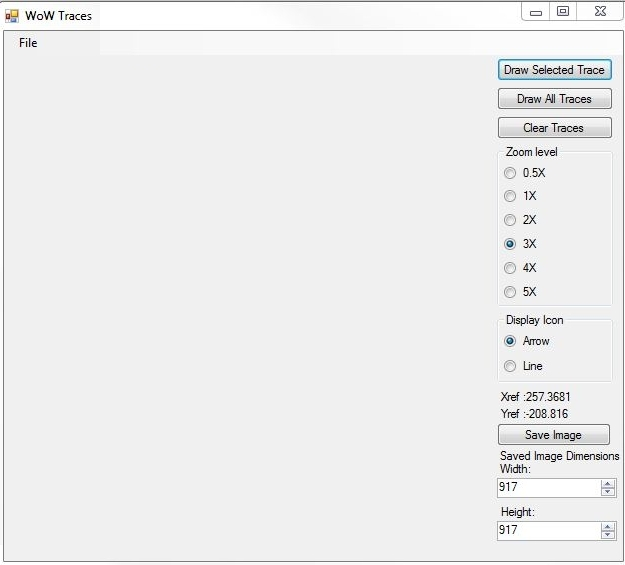
\includegraphics[scale = 0.8]{wowtraces1.jpg}	
\caption{The GUI of the log reading software}
\label{wowtraces}
\end{figure}


%Explain how the log reading program works. This could be a separate chapter?

%\section{Testing the Software}
%Several tests need to be done to ensure that the tracking software gathers accurate location data. This is done by going in game and comparing where NPCs and players are seen to where the software says they should be. This will give a general overview of whether the software works, but further testing is needed. Two characters need to log into the world simultaneously with each of them using the software. The coordinates of one character should be exactly the same on the two programs. The traces must then be tested by moving the character around and seeing if the trace on the other players tracking software reflects the same movements made. The data must then be logged, and the log reading program tested by redrawing the trace and seeing if it looks the same. 
%
%Larger scale testing then needs to be done by going into a capital city and capturing data and showing traces. The traces should then be compared to the layout of the city to see if the movement data makes logical sense. This is all done in chapter~\ref{results}. 

%Explain tests done to ensure that the software works as expected. Show proof and explain inconsistencies and mention latency.